%%----------------------------------------------------------------------------------------
%	PACKAGES AND THEMES
%----------------------------------------------------------------------------------------
\PassOptionsToPackage{table}{xcolor}
\documentclass[aspectratio=169,xcolor=dvipsnames,svgnames,x11names,fleqn]{beamer}
% \documentclass[aspectratio=169,xcolor=dvipsnames,fleqn]{beamer}

\usetheme{RedVelvet}

\usefonttheme[onlymath]{serif}
\newcommand{\showanswers}{yes}


\usepackage{xspace}
\usepackage{amsmath}
\usepackage{amssymb}
\usepackage{amsfonts}
\usepackage{color}
\usepackage{physics}
% \usepackage{mathbb}
\usepackage{rahul_math}
\usepackage{bigints}

\usepackage{graphicx} % Allows including images
\usepackage{booktabs} % Allows the use of \toprule, \midrule and \bottomrule in tables
\usepackage{tikz,pgfplots}

\usepackage{subfigure}
\usetikzlibrary{arrows}
\usepackage{minted}
\definecolor{LightGray}{gray}{0.9}
\definecolor{cream}{rgb}{0.92, 0.9, 0.55}
\definecolor{lightblue}{rgb}{0.68, 0.85, 0.9}


\usepackage{xcolor-material}
\usetikzlibrary{fit}
\usetikzlibrary{matrix}
\tikzset{%
apple/.pic={
    \fill [MaterialBrown] (-1/8,0)  arc (180:120:1 and 3/2) coordinate [pos=3/5] (@)-- ++(1/6,-1/7)  arc (120:180:5/4 and 3/2) -- cycle;
    \fill [MaterialLightGreen500] (0,-9/10)  .. controls ++(180:1/8) and ++(  0:1/4) .. (-1/3,  -1) .. controls ++(180:1/3) and ++(270:1/2) .. (  -1,   0) .. controls ++( 90:1/3) and ++(180:1/3) .. (-1/2, 3/4) .. controls ++(  0:1/8) and ++(135:1/8) .. (   0, 4/7)
    }
    }

\newcommand{\leftdoublequote}{\textcolor{blue}{\scalebox{3}{``}}}

\newcommand{\rightdoublequote}{\textcolor{blue}{\scalebox{3}{''}}}


\usepackage{textcomp}
\usepackage{fontawesome}
\usepackage{tikz,pgfplots}
\usetikzlibrary{shapes.callouts}
\usetikzlibrary{arrows}
\usetikzlibrary{shapes.geometric, positioning}
\pgfplotsset{compat=1.8} % or newest version

\usetikzlibrary{positioning}


\usepackage{bm}
\usepackage{relsize}



\tikzset{basic/.style={draw,fill=MediumBlue!20,text width=1em,text badly centered}}
\tikzset{input/.style={basic,circle}}
\tikzset{weights/.style={basic,rectangle}}
\tikzset{functions/.style={basic,circle,fill=MediumBlue!10}}



\usepackage{listofitems} % for \readlist to create arrays
\tikzstyle{mynode}=[thick,draw=MediumBlue,fill=MediumBlue!20,circle,minimum size=22]


\usepackage{overpic}

%----------------------------------------------------------------------------------------
%	TITLE PAGE
%----------------------------------------------------------------------------------------

\usepackage{tikz-qtree,tikz-qtree-compat}
\usetikzlibrary{tikzmark}
\usetikzlibrary{calc}

\usetikzlibrary{fit}
\tikzset{%
apple/.pic={
    \fill [MaterialBrown] (-1/8,0)  arc (180:120:1 and 3/2) coordinate [pos=3/5] (@)-- ++(1/6,-1/7)  arc (120:180:5/4 and 3/2) -- cycle;
    \fill [MaterialLightGreen500] (0,-9/10)  .. controls ++(180:1/8) and ++(  0:1/4) .. (-1/3,  -1) .. controls ++(180:1/3) and ++(270:1/2) .. (  -1,   0) .. controls ++( 90:1/3) and ++(180:1/3) .. (-1/2, 3/4) .. controls ++(  0:1/8) and ++(135:1/8) .. (   0, 4/7)
}
}
\usepackage{tikz-qtree,tikz-qtree-compat}
\usetikzlibrary{tikzmark}
\usetikzlibrary{calc}

\usetikzlibrary{positioning}


\usepackage{bm}
\usepackage{relsize}



\tikzset{basic/.style={draw,fill=MediumBlue!20,text width=1em,text badly centered}}
\tikzset{input/.style={basic,circle}}
\tikzset{weights/.style={basic,rectangle}}
\tikzset{functions/.style={basic,circle,fill=MediumBlue!10}}



\usepackage{listofitems} % for \readlist to create arrays
\tikzstyle{mynode}=[thick,draw=MediumBlue,fill=MediumBlue!20,circle,minimum size=22]


\newmdenv[
backgroundcolor=androidYellowLight,
linecolor=androidYellow,
linewidth=0.5pt,
roundcorner=10pt,
skipabove=\baselineskip,
skipbelow=\baselineskip
]{MintedFrame}

% Set minted options
\setminted{
fontsize=\footnotesize,
breaklines=true,
autogobble,
linenos,
frame=none
}


\title[CPE 487/587: Deep Learning]{CPE 486/586: Deep Learning for Engineering Applications} % The short title appears at the bottom of every slide, the full title is only on the title page
\subtitle{04 Training Neural Networks  and Computational Thinking}

\author[Rahul Bhadani] {{\Large \textbf{Rahul Bhadani}}}

\institute[UAH] % Your institution as it will appear on the bottom of every slide, maybe shorthand to save space
{
    Electrical \& Computer Engineering,  The University of Alabama in Huntsville
}
\date

% \titlegraphic{
%    \includegraphics[width=0.4\linewidth]{figures/UAH_primary.png}
% }

\begin{document}

%-------------------------------------------------
\begin{frame}
    \titlepage
\end{frame}

%-------------------------------------------------
\begin{frame}{Outline}
    \backgroundtableofcontents
\end{frame}


\section{Recap}

\begin{frame}
    \sectionpage
\end{frame}


\begin{frame}{Linear Layer}

\begin{columns}
\column{0.45\linewidth}


\begin{tikzpicture}[
    % Define styles for the nodes
    input_node/.style={circle, draw=black, fill=blue!30, thick, minimum size=1cm},
    output_node/.style={circle, draw=black, fill=orange!40, thick, minimum size=1cm},
    arrow/.style={-Stealth, thick}
]

    % Input Nodes (x1, x2)
    \node[input_node] (x1) at (0, 3) {$x_1$};
    \node[input_node] (x2) at (0, 1) {$x_2$};
    
    % Ellipsis (Vertical dots)
    \node at (0, -0.2) {\Huge $\vdots$};
    
    % Input Node (xN)
    \node[input_node] (xd) at (0, -1.5) {$x_d$};
    
    % Output Node (y)
    \node[output_node] (y) at (4, 0.75) {$y$};

    % Connections and Labels
    \draw[arrow] (x1) -- (y) node[midway, above right] {$w_1$};
    \draw[arrow] (x2) -- (y) node[midway, above] {$w_2$};
    \draw[arrow] (xd) -- (y) node[midway, below left] {$w_d$};

\end{tikzpicture}


\column{0.45\linewidth}

\pause 

\begin{align*}
y = \sum_{i = 1}^n w_i x_i
\end{align*}


\pause 

\begin{align*}
\wbf = \begin{bmatrix}
w_1 \\ w_2 \\ \vdots \\ w_d
\end{bmatrix} \quad \xbf = \begin{bmatrix}
x_1 & x_2 & \cdots & x_d
\end{bmatrix} 
\end{align*}

\pause 

\begin{align*}
\Rightarrow y = \xbf \wbf
\end{align*}
\end{columns}



\end{frame}



\begin{frame}{Linear Layer: Case of Hidden Layer}

\footnotesize 

\begin{columns}

\column{0.40\linewidth}
\begin{tikzpicture}[
    % Define styles for the nodes
    input_node/.style={circle, draw=black, fill=blue!30, thick, minimum size=1.1cm, inner sep=0pt},
    output_node/.style={circle, draw=black, fill=orange!40, thick, minimum size=1.1cm, inner sep=0pt},
    arrow/.style={-Stealth, thick}
]

    % Input Layer Nodes (x1, x2, ... xn)
    \node[input_node] (x1) at (0, 4) {$x_1$};
    \node[input_node] (x2) at (0, 2) {$x_2$};
    \node at (0, 0.5) {\Huge $\vdots$};
    \node[input_node] (xd) at (0, -1) {$x_d$};
    
    % Output Layer Nodes (z1, ... zM)
    \node[output_node] (z1) at (4, 3) {$z_1$};
    \node at (4, 1.5) {\Huge $\vdots$};
    \node[output_node] (zm) at (4, 0) {$z_m$};

    % Connections from x1
    \draw[arrow] (x1) -- (z1) node[midway, above, sloped] {$w_{11}$};
    \draw[arrow] (x1) -- (zm) node[pos=0.45, right] {$w_{1m}$};

    % Connections from x2
    \draw[arrow] (x2) -- (z1) node[pos=0.2, above] {$w_{21}$};
    \draw[arrow] (x2) -- (zm) node[pos=0.4, left] {$w_{2m}$};

    % Connections from xN
    \draw[arrow] (xd) -- (z1) node[pos=0.3, left] {$w_{d1}$};
    \draw[arrow] (xd) -- (zm) node[midway, below, sloped] {$w_{dm}$};

\end{tikzpicture}

\column{0.55\linewidth}

\pause 
\begin{align*}
z_m = \sum_{i = 1}^n x_i w_{im}
\end{align*}

\pause 

\begin{align*}
\zbf = \begin{bmatrix}
z_1 & z_2 & \vdots & z_m
\end{bmatrix}_{1 \times m} 
\end{align*}

\begin{align*}  W  = \begin{bmatrix}
w_{11} & w_{12} & \cdots & w_{1m}\\
w_{21} & w_{22} & \cdots & w_{2m}\\
\vdots & \vdots & \vdots & \vdots \\
w_{d1} & w_{m2} & \cdots & w_{dm}
\end{bmatrix}_{d \times m} \quad  \xbf = \begin{bmatrix}
x_1 & x_2 & \cdots & x_d
\end{bmatrix}_{1\times d}
\end{align*}

\pause

\begin{align*}
\Rightarrow \zbf = \xbf W
\end{align*}

\end{columns}

\end{frame}


\begin{frame}{Linear Layer: Case of Hidden Layer}

\footnotesize 

\begin{columns}

\column{0.40\linewidth}
\begin{tikzpicture}[
    % Define styles for the nodes
    input_node/.style={circle, draw=black, fill=blue!30, thick, minimum size=1.1cm, inner sep=0pt},
    output_node/.style={circle, draw=black, fill=orange!40, thick, minimum size=1.1cm, inner sep=0pt},
    arrow/.style={-Stealth, thick}
]

    % Input Layer Nodes (x1, x2, ... xn)
    \node[input_node] (x1) at (0, 4) {$x_1$};
    \node[input_node] (x2) at (0, 2) {$x_2$};
    \node at (0, 0.5) {\Huge $\vdots$};
    \node[input_node] (xd) at (0, -1) {$x_d$};
    
    % Output Layer Nodes (z1, ... zM)
    \node[output_node] (z1) at (4, 3) {$z_1$};
    \node at (4, 1.5) {\Huge $\vdots$};
    \node[output_node] (zm) at (4, 0) {$z_m$};

    % Connections from x1
    \draw[arrow] (x1) -- (z1) node[midway, above, sloped] {$w_{11}$};
    \draw[arrow] (x1) -- (zm) node[pos=0.45, right] {$w_{1m}$};

    % Connections from x2
    \draw[arrow] (x2) -- (z1) node[pos=0.2, above] {$w_{21}$};
    \draw[arrow] (x2) -- (zm) node[pos=0.4, left] {$w_{2m}$};

    % Connections from xN
    \draw[arrow] (xd) -- (z1) node[pos=0.3, left] {$w_{d1}$};
    \draw[arrow] (xd) -- (zm) node[midway, below, sloped] {$w_{dm}$};

\end{tikzpicture}

\column{0.55\linewidth}

That was the case of one sample, if we consider $n$ sample, then?


\pause

\begin{align*}
X = \begin{bmatrix}
x_{11} & x_{12} & \cdots & x_{1d}\\
x_{21} & x_{22} & \cdots & x_{2d}\\
\vdots & \vdots & \vdots & \vdots\\
x_{n1} & x_{n2} & \cdots & x_{nd}\\
\end{bmatrix}
\end{align*}

\pause

\begin{align*}
\Rightarrow Z = XW
\end{align*}

\end{columns}

\end{frame}

\begin{frame}{Nonlinear Operation}

\Large

\center

\begin{align*}
A = \sigma(Z)
\end{align*}

which will use elementwise operation.

\end{frame}



\section{Training a Neural Network}

\begin{frame}
    \sectionpage
\end{frame}

\begin{frame}{How to Train your Neural Network}

\begin{center}
\includegraphics[width=0.4\linewidth]{figures/how_to_train_your_nn.jpg}

\tiny 
Image generation from Google Gemini.
\end{center}

\end{frame}


\begin{frame}{Training a Neural Network}

Some criteria to consider:

\footnotesize


\begin{columns}
    \column{0.5\linewidth}

    \begin{enumerate}
\item Data Preprocessing: Normalization/Standardization
%\item Feature Engineering
\item Batch Size
\item Batch Normalization
\item Dropout
\item Early-Stopping
\item Learning-Rate Scheduling
\item Optimizer Selection
    \end{enumerate}

    \column{0.5\linewidth}
\begin{enumerate}
    \setcounter{enumi}{7}
    \item Weight Initialization
\item Activation Functions
\item Network Depth \& Width
\item Skip/Residual Connections
\item Regularization
\item Loss Functions
\item Gradient Clipping
\item Warm-Up Scheduling
\end{enumerate}

\end{columns}



\end{frame}

\subsection{Data Preprocessing}

\begin{frame}
    \subsectionpage
\end{frame}

\begin{frame}{Imputing Missing Values}


\begin{facts}{Definition}

The process of filling miss values or correct known errors is called \textbf{imputation}.

\end{facts}

\tiny

\begin{figure}[h]
\centering
\begin{tikzpicture}[scale=0.9]
    % Define colors
    \definecolor{headerBg}{RGB}{200, 220, 255}
    \definecolor{nanColor}{RGB}{255, 200, 200}
    \definecolor{dataColor}{RGB}{240, 248, 255}
    
    % Table parameters
    \def\cellw{1.2}
    \def\cellh{0.6}
    \def\sx{2}
    \def\sy{0}
    
    % ===== HEADER ROW =====
    \draw[fill=headerBg, draw=black, line width=1pt] 
        (\sx + 1*\cellw, \sy) rectangle (\sx + 2*\cellw, \sy + \cellh);
    \node at (\sx + 1.5*\cellw, \sy + \cellh/2) {\small $x_1$};
    
    \draw[fill=headerBg, draw=black, line width=1pt] 
        (\sx + 2*\cellw, \sy) rectangle (\sx + 3*\cellw, \sy + \cellh);
    \node at (\sx + 2.5*\cellw, \sy + \cellh/2) {\small $x_2$};
    
    \draw[fill=headerBg, draw=black, line width=1pt] 
        (\sx + 3*\cellw, \sy) rectangle (\sx + 4*\cellw, \sy + \cellh);
    \node at (\sx + 3.5*\cellw, \sy + \cellh/2) {\small $x_3$};
    
    \draw[fill=headerBg, draw=black, line width=1pt] 
        (\sx + 4*\cellw, \sy) rectangle (\sx + 5*\cellw, \sy + \cellh);
    \node at (\sx + 4.5*\cellw, \sy + \cellh/2) {\small $x_4$};
    
    \draw[fill=headerBg, draw=black, line width=1pt] 
        (\sx + 5*\cellw, \sy) rectangle (\sx + 6*\cellw, \sy + \cellh);
    \node at (\sx + 5.5*\cellw, \sy + \cellh/2) {\small $x_5$};
    
    % ===== ROW 0: Sample 0 =====
    \node[anchor=east, font=\small\bfseries] at (\sx - 0.3, \sy - 1*\cellh + \cellh/2) {Sample 0};
    
    \draw[fill=dataColor, draw=black, line width=0.5pt] (\sx + 1*\cellw, \sy - 1*\cellh) rectangle (\sx + 2*\cellw, \sy - 1*\cellh + \cellh);
    \node at (\sx + 1.5*\cellw, \sy - 1*\cellh + \cellh/2) {\footnotesize 2.3};
    
    \draw[fill=dataColor, draw=black, line width=0.5pt] (\sx + 2*\cellw, \sy - 1*\cellh) rectangle (\sx + 3*\cellw, \sy - 1*\cellh + \cellh);
    \node at (\sx + 2.5*\cellw, \sy - 1*\cellh + \cellh/2) {\footnotesize 4.1};
    
    \draw[fill=nanColor, draw=black, line width=0.5pt] (\sx + 3*\cellw, \sy - 1*\cellh) rectangle (\sx + 4*\cellw, \sy - 1*\cellh + \cellh);
    \node at (\sx + 3.5*\cellw, \sy - 1*\cellh + \cellh/2) {\footnotesize NaN};
    
    \draw[fill=dataColor, draw=black, line width=0.5pt] (\sx + 4*\cellw, \sy - 1*\cellh) rectangle (\sx + 5*\cellw, \sy - 1*\cellh + \cellh);
    \node at (\sx + 4.5*\cellw, \sy - 1*\cellh + \cellh/2) {\footnotesize 3.7};
    
    \draw[fill=dataColor, draw=black, line width=0.5pt] (\sx + 5*\cellw, \sy - 1*\cellh) rectangle (\sx + 6*\cellw, \sy - 1*\cellh + \cellh);
    \node at (\sx + 5.5*\cellw, \sy - 1*\cellh + \cellh/2) {\footnotesize 1.9};
    
    % ===== ROW 1: Sample 1 =====
    \node[anchor=east, font=\small\bfseries] at (\sx - 0.3, \sy - 2*\cellh + \cellh/2) {Sample 1};
    
    \draw[fill=dataColor, draw=black, line width=0.5pt] (\sx + 1*\cellw, \sy - 2*\cellh) rectangle (\sx + 2*\cellw, \sy - 2*\cellh + \cellh);
    \node at (\sx + 1.5*\cellw, \sy - 2*\cellh + \cellh/2) {\footnotesize 5.2};
    
    \draw[fill=nanColor, draw=black, line width=0.5pt] (\sx + 2*\cellw, \sy - 2*\cellh) rectangle (\sx + 3*\cellw, \sy - 2*\cellh + \cellh);
    \node at (\sx + 2.5*\cellw, \sy - 2*\cellh + \cellh/2) {\footnotesize NaN};
    
    \draw[fill=dataColor, draw=black, line width=0.5pt] (\sx + 3*\cellw, \sy - 2*\cellh) rectangle (\sx + 4*\cellw, \sy - 2*\cellh + \cellh);
    \node at (\sx + 3.5*\cellw, \sy - 2*\cellh + \cellh/2) {\footnotesize 2.8};
    
    \draw[fill=dataColor, draw=black, line width=0.5pt] (\sx + 4*\cellw, \sy - 2*\cellh) rectangle (\sx + 5*\cellw, \sy - 2*\cellh + \cellh);
    \node at (\sx + 4.5*\cellw, \sy - 2*\cellh + \cellh/2) {\footnotesize 1.5};
    
    \draw[fill=dataColor, draw=black, line width=0.5pt] (\sx + 5*\cellw, \sy - 2*\cellh) rectangle (\sx + 6*\cellw, \sy - 2*\cellh + \cellh);
    \node at (\sx + 5.5*\cellw, \sy - 2*\cellh + \cellh/2) {\footnotesize 4.3};
    
    % ===== ROW 2: Sample 2 =====
    \node[anchor=east, font=\small\bfseries] at (\sx - 0.3, \sy - 3*\cellh + \cellh/2) {Sample 2};
    
    \draw[fill=dataColor, draw=black, line width=0.5pt] (\sx + 1*\cellw, \sy - 3*\cellh) rectangle (\sx + 2*\cellw, \sy - 3*\cellh + \cellh);
    \node at (\sx + 1.5*\cellw, \sy - 3*\cellh + \cellh/2) {\footnotesize 1.1};
    
    \draw[fill=dataColor, draw=black, line width=0.5pt] (\sx + 2*\cellw, \sy - 3*\cellh) rectangle (\sx + 3*\cellw, \sy - 3*\cellh + \cellh);
    \node at (\sx + 2.5*\cellw, \sy - 3*\cellh + \cellh/2) {\footnotesize 3.4};
    
    \draw[fill=dataColor, draw=black, line width=0.5pt] (\sx + 3*\cellw, \sy - 3*\cellh) rectangle (\sx + 4*\cellw, \sy - 3*\cellh + \cellh);
    \node at (\sx + 3.5*\cellw, \sy - 3*\cellh + \cellh/2) {\footnotesize 2.6};
    
    \draw[fill=nanColor, draw=black, line width=0.5pt] (\sx + 4*\cellw, \sy - 3*\cellh) rectangle (\sx + 5*\cellw, \sy - 3*\cellh + \cellh);
    \node at (\sx + 4.5*\cellw, \sy - 3*\cellh + \cellh/2) {\footnotesize NaN};
    
    \draw[fill=dataColor, draw=black, line width=0.5pt] (\sx + 5*\cellw, \sy - 3*\cellh) rectangle (\sx + 6*\cellw, \sy - 3*\cellh + \cellh);
    \node at (\sx + 5.5*\cellw, \sy - 3*\cellh + \cellh/2) {\footnotesize 5.1};
    
    % ===== ROW 3: Sample 3 =====
    \node[anchor=east, font=\small\bfseries] at (\sx - 0.3, \sy - 4*\cellh + \cellh/2) {Sample 3};
    
    \draw[fill=nanColor, draw=black, line width=0.5pt] (\sx + 1*\cellw, \sy - 4*\cellh) rectangle (\sx + 2*\cellw, \sy - 4*\cellh + \cellh);
    \node at (\sx + 1.5*\cellw, \sy - 4*\cellh + \cellh/2) {\footnotesize NaN};
    
    \draw[fill=dataColor, draw=black, line width=0.5pt] (\sx + 2*\cellw, \sy - 4*\cellh) rectangle (\sx + 3*\cellw, \sy - 4*\cellh + \cellh);
    \node at (\sx + 2.5*\cellw, \sy - 4*\cellh + \cellh/2) {\footnotesize 2.2};
    
    \draw[fill=dataColor, draw=black, line width=0.5pt] (\sx + 3*\cellw, \sy - 4*\cellh) rectangle (\sx + 4*\cellw, \sy - 4*\cellh + \cellh);
    \node at (\sx + 3.5*\cellw, \sy - 4*\cellh + \cellh/2) {\footnotesize 4.0};
    
    \draw[fill=dataColor, draw=black, line width=0.5pt] (\sx + 4*\cellw, \sy - 4*\cellh) rectangle (\sx + 5*\cellw, \sy - 4*\cellh + \cellh);
    \node at (\sx + 4.5*\cellw, \sy - 4*\cellh + \cellh/2) {\footnotesize 3.3};
    
    \draw[fill=dataColor, draw=black, line width=0.5pt] (\sx + 5*\cellw, \sy - 4*\cellh) rectangle (\sx + 6*\cellw, \sy - 4*\cellh + \cellh);
    \node at (\sx + 5.5*\cellw, \sy - 4*\cellh + \cellh/2) {\footnotesize 2.9};
    
    % ===== ROW 4: Sample 4 =====
    \node[anchor=east, font=\small\bfseries] at (\sx - 0.3, \sy - 5*\cellh + \cellh/2) {Sample 4};
    
    \draw[fill=dataColor, draw=black, line width=0.5pt] (\sx + 1*\cellw, \sy - 5*\cellh) rectangle (\sx + 2*\cellw, \sy - 5*\cellh + \cellh);
    \node at (\sx + 1.5*\cellw, \sy - 5*\cellh + \cellh/2) {\footnotesize 3.5};
    
    \draw[fill=dataColor, draw=black, line width=0.5pt] (\sx + 2*\cellw, \sy - 5*\cellh) rectangle (\sx + 3*\cellw, \sy - 5*\cellh + \cellh);
    \node at (\sx + 2.5*\cellw, \sy - 5*\cellh + \cellh/2) {\footnotesize 1.8};
    
    \draw[fill=dataColor, draw=black, line width=0.5pt] (\sx + 3*\cellw, \sy - 5*\cellh) rectangle (\sx + 4*\cellw, \sy - 5*\cellh + \cellh);
    \node at (\sx + 3.5*\cellw, \sy - 5*\cellh + \cellh/2) {\footnotesize 2.1};
    
    \draw[fill=dataColor, draw=black, line width=0.5pt] (\sx + 4*\cellw, \sy - 5*\cellh) rectangle (\sx + 5*\cellw, \sy - 5*\cellh + \cellh);
    \node at (\sx + 4.5*\cellw, \sy - 5*\cellh + \cellh/2) {\footnotesize 4.5};
    
    \draw[fill=nanColor, draw=black, line width=0.5pt] (\sx + 5*\cellw, \sy - 5*\cellh) rectangle (\sx + 6*\cellw, \sy - 5*\cellh + \cellh);
    \node at (\sx + 5.5*\cellw, \sy - 5*\cellh + \cellh/2) {\footnotesize NaN};
    
    % ===== ROW 5: Sample 5 =====
    \node[anchor=east, font=\small\bfseries] at (\sx - 0.3, \sy - 6*\cellh + \cellh/2) {Sample 5};
    
    \draw[fill=dataColor, draw=black, line width=0.5pt] (\sx + 1*\cellw, \sy - 6*\cellh) rectangle (\sx + 2*\cellw, \sy - 6*\cellh + \cellh);
    \node at (\sx + 1.5*\cellw, \sy - 6*\cellh + \cellh/2) {\footnotesize 2.7};
    
    \draw[fill=dataColor, draw=black, line width=0.5pt] (\sx + 2*\cellw, \sy - 6*\cellh) rectangle (\sx + 3*\cellw, \sy - 6*\cellh + \cellh);
    \node at (\sx + 2.5*\cellw, \sy - 6*\cellh + \cellh/2) {\footnotesize 3.9};
    
    \draw[fill=nanColor, draw=black, line width=0.5pt] (\sx + 3*\cellw, \sy - 6*\cellh) rectangle (\sx + 4*\cellw, \sy - 6*\cellh + \cellh);
    \node at (\sx + 3.5*\cellw, \sy - 6*\cellh + \cellh/2) {\footnotesize NULL};
    
    \draw[fill=dataColor, draw=black, line width=0.5pt] (\sx + 4*\cellw, \sy - 6*\cellh) rectangle (\sx + 5*\cellw, \sy - 6*\cellh + \cellh);
    \node at (\sx + 4.5*\cellw, \sy - 6*\cellh + \cellh/2) {\footnotesize 1.2};
    
    \draw[fill=dataColor, draw=black, line width=0.5pt] (\sx + 5*\cellw, \sy - 6*\cellh) rectangle (\sx + 6*\cellw, \sy - 6*\cellh + \cellh);
    \node at (\sx + 5.5*\cellw, \sy - 6*\cellh + \cellh/2) {\footnotesize 4.6};
    
    % ===== FEATURE INDEX ARROW (above) =====
    \draw[-{Latex[length=3mm, width=2mm]}, line width=2pt, color=blue] 
        (\sx + 1.5*\cellw, \sy + 1.5*\cellh) -- (\sx + 5.5*\cellw, \sy + 1.5*\cellh);
    \node[anchor=south, font=\large, color=blue] 
        at (\sx + 3.5*\cellw, \sy + 1.8*\cellh) {Feature Index};
    
    % ===== SAMPLE INDEX ARROW (left side, rotated) =====
    \draw[-{Latex[length=3mm, width=2mm]}, line width=2pt, color=red] 
        (\sx + 0.8, \sy - 0.5*\cellh) -- (\sx + 0.8, \sy - 5.5*\cellh);
    \node[rotate=90, anchor=south, font=\large, color=red] 
        at (\sx + 0.5, \sy - 3*\cellh) {Sample Index};
    
    % ===== LEGEND BOX =====
    \begin{scope}[xshift=12cm, yshift=-1cm]
        \draw[fill=white, draw=black, line width=1.5pt, rounded corners=3pt] 
            (0, 0) rectangle (4, 2.5);
        
        \node[anchor=west, font=\bfseries] at (0.2, 2) {Legend:};
        
        \draw[fill=headerBg, draw=black] (0.2, 1.5) rectangle (0.6, 1.8);
        \node[anchor=west, font=\small] at (0.8, 1.65) {Feature header};
        
        \draw[fill=dataColor, draw=black] (0.2, 1.0) rectangle (0.6, 1.3);
        \node[anchor=west, font=\small] at (0.8, 1.15) {Valid data};
        
        \draw[fill=nanColor, draw=black] (0.2, 0.5) rectangle (0.6, 0.8);
        \node[anchor=west, font=\small] at (0.8, 0.65) {Missing (NaN)};
    \end{scope}
    
    
    
\end{tikzpicture}
\caption{Data Table Structure: Features as Columns, Samples as Rows. 
Red cells indicate missing values (NaN) that require imputation before model training.}
\end{figure}


\end{frame}


\begin{frame}{Common Types of Missing Values}

\begin{enumerate}

\item Missing Completely at Random (MCAR), i.e. the probability
of being missing is not related to the data and is only dependent on some parameter $\phi$.

\item Missing at Random (MAR), i.e., the missingness probability is only related to the observed variables in the data.

\item Missing not at random (MNAR), neither of the above, and  the missingness probability is related to missing values of the
incomplete variable, which are unknown to us, even after conditioning on observed information

\end{enumerate}

\end{frame}


\begin{frame}{Common Imputation Methods}

\begin{enumerate}

\item Get rid of those samples where missing \# features exceed certain number (or percentage)
\item Get rid of feaures where \# missing values exceed certai numbers (or percentage)
\item Sample Mean (only for continuous data)
\item Sample Median (only for continuous data) 
\item k-Nearest Neighbors (kNN) imputation
\item Expectation-Maximization (EM) imputation
\item Bayesian Approach
\end{enumerate}

\begin{tblock}{}
Mean and median approach or anything similar would fail to quantify uncertainty in the estimated missing value.
\end{tblock}

\end{frame}

\begin{frame}{Bayesian Estimation for Missing Data}

\begin{gradbox}{}

\begin{enumerate}

\item Model your data first (probabilistic modeling): e.g. normal distribution.

\item Compute prior distribution over uknown parameters.
\item Calculate posterior: update the prior using observed data as (Bayes' Theorem in the play). This gives a posterior distribution over model parameters and missing values.
\item Draw samples using Markov Chain Monte Carlo simulation that will be plausible missing values.

\begin{center}
{\bf\color{SeaGreen4}Under a Bayesian framework, missing observations can be thought of as any other parameter in the model whose distribution needs to be determined.}
\end{center}

\end{enumerate}
\end{gradbox} 
 
\end{frame}

\begin{frame}{Bayesian Framework}

\small

\begin{tcolorbox}[title=Posterior Distribution, colframe=pink]

\begin{align*}
p(\boldsymbol{\theta} \mid X) = \frac{p(\mathbf{X} \mid \boldsymbol{\theta}) \, p(\boldsymbol{\theta})}{\int_{-\infty}^{\infty} p(\mathbf{X} \mid \boldsymbol{\theta}) \, p(\boldsymbol{\theta}) \, d\boldsymbol{\theta}}  \propto p(\mathbf{X} \mid \boldsymbol{\theta}) \, p(\boldsymbol{\theta})
\end{align*}

$p(\mathbf{X} \mid \boldsymbol{\theta})$ is likelihood, $p(\boldsymbol{\theta})$ is prior.



\end{tcolorbox}

\begin{align*}
p(\mathbf{X}_{mis} \mid \mathbf{X}_{obs}) = \int p(\mathbf{X}_{mis} \mid \mathbf{X}_{obs}, \boldsymbol{\theta}) \, p(\boldsymbol{\theta} \mid \mathbf{X}_{obs}) \, d\boldsymbol{\theta}.
\end{align*}

Calculating posterior is hard, so we use Monte Carlo methods (Markov Chain Monte Carlo (MCMC)).

\footnotesize 

An example code for MCMC imputation using PyMC is available at {\url{https://www.pymc.io/projects/examples/en/latest/howto/Missing_Data_Imputation.html}}
\end{frame}


\begin{frame}{Normalization/Standardization}

\begin{tcolorbox}[title=Definition, colframe=pink, colback=NavajoWhite1]
In simpler terms: adjusting values measured on different scales to a common scale is \textbf{Normalization}.

\bigskip

Otherwise, aligning entire probability distribution of adjusted values is \textbf{Normalization}.


\end{tcolorbox}


\begin{columns}
    \column{0.5\linewidth}

    \begin{tcolorbox}[colframe=lightblue, title=Standard Normalization]
        \begin{align*}
            \xhat = \frac{x - \mu}{\sigma}
        \end{align*}
    \end{tcolorbox}

    \column{0.5\linewidth}

    \begin{tcolorbox}[colframe=Green!60, title=Minmax Normalization]
        \begin{align*}
            \xhat = \frac{x - x_{min}}{ x_{max} -  x_{min}}
        \end{align*}
    \end{tcolorbox}
    
\end{columns}


\end{frame}


\subsection{Impact of Batch Size in the Training Process}

\begin{frame}
    \subsectionpage
\end{frame}


\begin{frame}{Batch Size}

    \begin{tcolorbox}[title=Definition, colframe=Orange!30, colback=Green!10]
    The number of samples passed through the neural network simultaneously is called \textbf{batch size}.
    \end{tcolorbox}
    
    Determining a suitable batch size is an important consideration to the training process, as it may influence the learning rate of the model. 
    
    \begin{center}
    \begin{align*}
    \wbf = \wbf - \eta \frac{1}{m}\sum_{i=1}^m \nabla_\wbf \Lcal_i(\wbf)
    \end{align*}
    \end{center}
    

    $m$ is the batch size.

\end{frame}

\begin{frame}{}
    
    \begin{center}
        \begin{forest}{}
            \LARGE \centering
        How does the batch size affect training?
        \end{forest}

    \end{center}
    
\end{frame}

\begin{frame}{Stochastic Gradient Descent and Batch Size}
    
    \Large 
    {\faQuestionCircle~~ What's problem if we use entire training set for gradient descent? }

    \pause 

    \vspace{10pt}

    \begin{tblock}{}
        Stochastic gradient descent provides approximation of true gradients using one sample at a time after shuffling the training sample and pick one training sample to update the weights. It optionally adds a small noise to the gradient calculation.
    \end{tblock}
    

\end{frame}

\begin{frame}{Mini Batch}
    
    Single sample gradient calculation can be very slow, so we can choose more than one sample at a time (but not all of them). This is called \textbf{mini batch}.

\end{frame}

\begin{frame}{Suggested Reading}

    \large 
    \begin{enumerate}
        \item Masters, Dominic, and Carlo Luschi. \textbf{"Revisiting small batch training for deep neural networks."} arXiv preprint arXiv:1804.07612 (2018).
        \item You, Yang, Yuhui Wang, Huan Zhang, Zhao Zhang, James Demmel, and Cho-Jui Hsieh. \textbf{"The limit of the batch size."} arXiv preprint arXiv:2006.08517 (2020).
        \item Smith, Samuel L., Pieter-Jan Kindermans, Chris Ying, and Quoc V. Le. \textbf{"Don't decay the learning rate, increase the batch size."} arXiv preprint arXiv:1711.00489 (2017).
    \end{enumerate}
    
\end{frame}

\begin{frame}{Batch Normalization}

    Normalization applied per batch:

    \begin{align*}
        \hat{\xbf}_i = \frac{\xbf_i - \mu_{\Bcal}}{\sqrt{\sigma^2_\Bcal + \epsilon}}
    \end{align*}
    
    $ \mu_{\Bcal}$ batchwise mean, $\sigma^2_\Bcal$ is batchwise variance, and $\epsilon$ is to avoid numerical instability.
\end{frame}

\begin{frame}{Batch Normalization}
    But why Batch Normalization?

    \pause 

    \begin{enumerate}
        \item Batch Normalization smoothened out the loss landscape.
        \item Gradients become more reliable and predictive.
    \end{enumerate}

    \bigskip

    \small

\textbf{Reading:}

    \footnotesize


\begin{enumerate}
    \item Santurkar, Shibani, Dimitris Tsipras, Andrew Ilyas, and Aleksander Madry. \textbf{"How does batch normalization help optimization?."} Advances in neural information processing systems 31 (2018).
    \item Section 3.3 of Huang, Lei. Normalization Techniques in Deep Learning. Cham: Springer, 2022.
\end{enumerate}

\end{frame}


\subsection{Preventing Overfitting and Regularization}

\begin{frame}
    \subsectionpage
\end{frame}


%------------------------------------------------
\begin{frame}{Dropout}

\begin{tblock}{Dropout: A new way to regularize a network}
\begin{itemize}
    \item The central idea behind {\em\color{MediumBlue}dropout} is to randomly dropout nodes in the neural network with a probability $p$. After the nodes are ``dropped out'' the remain network is a subnetwork of the original. 
    \item Dropout has been shown to work quite well at preventing overfitting and allowing the network to find a good local minimum. 
    \item {\bf\color{MediumRed}Recommendation}: Use dropout! 
\end{itemize}
\end{tblock}
{\footnotesize
Nitish Srivastava, Geoffrey Hinton, Alex Krizhevsky, Ilya Sutskever, Ruslan Salakhutdinov, ``Dropout: A Simple Way to Prevent Neural Networks from Overfitting,'' {\em Journal of Machine Learning Research}, 15(56):1929--1958, 2014.}
\end{frame}


%------------------------------------------------
\begin{frame}{Dropout in a Neural Network}

\begin{center}
    
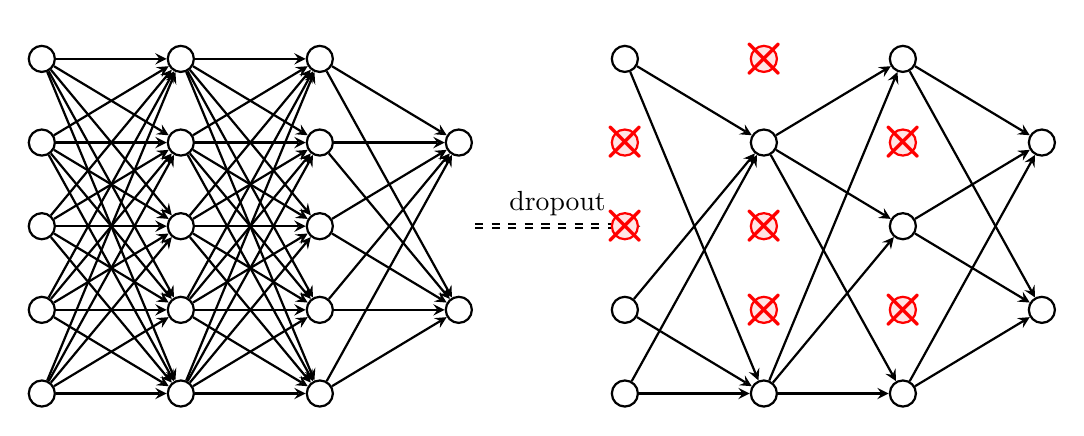
\begin{tikzpicture}

	\node[circle, draw, thick] (i1) {};
	\node[circle, draw, thick, above=2em of i1] (i2) {};
	\node[circle, draw, thick, above=2em of i2] (i3) {};
	\node[circle, draw, thick, below=2em of i1] (i4) {};
	\node[circle, draw, thick, below=2em of i4] (i5) {};
	
	\node[circle, draw, thick, right=4em of i1] (h1) {};
	\node[circle, draw, thick, right=4em of i2] (h2) {};
	\node[circle, draw, thick, right=4em of i3] (h3) {};
	\node[circle, draw, thick, right=4em of i4] (h4) {};
	\node[circle, draw, thick, right=4em of i5] (h5) {};
	
	\node[circle, draw, thick, right=4em of h1] (hh1) {};
	\node[circle, draw, thick, right=4em of h2] (hh2) {};
	\node[circle, draw, thick, right=4em of h3] (hh3) {};
	\node[circle, draw, thick, right=4em of h4] (hh4) {};
	\node[circle, draw, thick, right=4em of h5] (hh5) {};
	
	\node[circle, draw, thick, right=4em of hh2] (o1) {};
	\node[circle, draw, thick, right=4em of hh4] (o2) {};
	
	\draw[-stealth, thick] (i1) -- (h1);
	\draw[-stealth, thick] (i1) -- (h2);
	\draw[-stealth, thick] (i1) -- (h3);
	\draw[-stealth, thick] (i1) -- (h4);
	\draw[-stealth, thick] (i1) -- (h5);
	\draw[-stealth, thick] (i2) -- (h1);
	\draw[-stealth, thick] (i2) -- (h2);
	\draw[-stealth, thick] (i2) -- (h3);
	\draw[-stealth, thick] (i2) -- (h4);
	\draw[-stealth, thick] (i2) -- (h5);
	\draw[-stealth, thick] (i3) -- (h1);
	\draw[-stealth, thick] (i3) -- (h2);
	\draw[-stealth, thick] (i3) -- (h3);
	\draw[-stealth, thick] (i3) -- (h4);
	\draw[-stealth, thick] (i3) -- (h5);
	\draw[-stealth, thick] (i4) -- (h1);
	\draw[-stealth, thick] (i4) -- (h2);
	\draw[-stealth, thick] (i4) -- (h3);
	\draw[-stealth, thick] (i4) -- (h4);
	\draw[-stealth, thick] (i4) -- (h5);
	\draw[-stealth, thick] (i5) -- (h1);
	\draw[-stealth, thick] (i5) -- (h2);
	\draw[-stealth, thick] (i5) -- (h3);
	\draw[-stealth, thick] (i5) -- (h4);
	\draw[-stealth, thick] (i5) -- (h5);
	
	\draw[-stealth, thick] (h1) -- (hh1);
	\draw[-stealth, thick] (h1) -- (hh2);
	\draw[-stealth, thick] (h1) -- (hh3);
	\draw[-stealth, thick] (h1) -- (hh4);
	\draw[-stealth, thick] (h1) -- (hh5);
	\draw[-stealth, thick] (h2) -- (hh1);
	\draw[-stealth, thick] (h2) -- (hh2);
	\draw[-stealth, thick] (h2) -- (hh3);
	\draw[-stealth, thick] (h2) -- (hh4);
	\draw[-stealth, thick] (h2) -- (hh5);
	\draw[-stealth, thick] (h3) -- (hh1);
	\draw[-stealth, thick] (h3) -- (hh2);
	\draw[-stealth, thick] (h3) -- (hh3);
	\draw[-stealth, thick] (h3) -- (hh4);
	\draw[-stealth, thick] (h3) -- (hh5);
	\draw[-stealth, thick] (h4) -- (hh1);
	\draw[-stealth, thick] (h4) -- (hh2);
	\draw[-stealth, thick] (h4) -- (hh3);
	\draw[-stealth, thick] (h4) -- (hh4);
	\draw[-stealth, thick] (h4) -- (hh5);
	\draw[-stealth, thick] (h5) -- (hh1);
	\draw[-stealth, thick] (h5) -- (hh2);
	\draw[-stealth, thick] (h5) -- (hh3);
	\draw[-stealth, thick] (h5) -- (hh4);
	\draw[-stealth, thick] (h5) -- (hh5);
	
	
	\draw[-stealth, thick] (hh1) -- (o1);
	\draw[-stealth, thick] (hh1) -- (o2);
	\draw[-stealth, thick] (hh2) -- (o1);
	\draw[-stealth, thick] (hh2) -- (o2);
	\draw[-stealth, thick] (hh3) -- (o1);
	\draw[-stealth, thick] (hh3) -- (o2);
	\draw[-stealth, thick] (hh4) -- (o1);
	\draw[-stealth, thick] (hh4) -- (o2);
	\draw[-stealth, thick] (hh5) -- (o1);
	\draw[-stealth, thick] (hh5) -- (o2);
	
	\draw[-stealth, double, dashed, thick] (5.5,0) -- node[above] {dropout} (7.6, 0);
	
	
	%%% BOUNDARY %%%
	
	\node[circle, draw, thick, red, fill=red!10, right=10em of hh1] (i1) {};
	\node[circle, draw, thick, red, fill=red!10, above=2em of i1] (i2) {};
	\node[circle, draw, thick, above=2em of i2] (i3) {};
	\node[circle, draw, thick, below=2em of i1] (i4) {};
	\node[circle, draw, thick, below=2em of i4] (i5) {};
	
	\node[red] (icr) at (i1) {$\mathlarger{\mathlarger{\mathlarger{\mathlarger{\mathlarger{\bm{\times}}}}}}$};
	\node[red] (icr) at (i2) {$\mathlarger{\mathlarger{\mathlarger{\mathlarger{\mathlarger{\bm{\times}}}}}}$};
	
	\node[circle, draw, thick, red, fill=red!10, right=4em of i1] (h1) {};
	\node[circle, draw, thick, right=4em of i2] (h2) {};
	\node[circle, draw, thick, red, fill=red!10, right=4em of i3] (h3) {};
	\node[circle, draw, thick, red, fill=red!10, right=4em of i4] (h4) {};
	\node[circle, draw, thick, right=4em of i5] (h5) {};
	
	\node[red] (icr) at (h1) {$\mathlarger{\mathlarger{\mathlarger{\mathlarger{\mathlarger{\bm{\times}}}}}}$};
	\node[red] (icr) at (h3) {$\mathlarger{\mathlarger{\mathlarger{\mathlarger{\mathlarger{\bm{\times}}}}}}$};
	\node[red] (icr) at (h4) {$\mathlarger{\mathlarger{\mathlarger{\mathlarger{\mathlarger{\bm{\times}}}}}}$};
	
	\node[circle, draw, thick, right=4em of h1] (hh1) {};
	\node[circle, draw, thick, red, fill=red!10, right=4em of h2] (hh2) {};
	\node[circle, draw, thick, right=4em of h3] (hh3) {};
	\node[circle, draw, thick, red, fill=red!10, right=4em of h4] (hh4) {};
	\node[circle, draw, thick, right=4em of h5] (hh5) {};
	
	\node[red] (icr) at (hh2) {$\mathlarger{\mathlarger{\mathlarger{\mathlarger{\mathlarger{\bm{\times}}}}}}$};
	\node[red] (icr) at (hh4) {$\mathlarger{\mathlarger{\mathlarger{\mathlarger{\mathlarger{\bm{\times}}}}}}$};
	
	\node[circle, draw, thick, right=4em of hh2] (o1) {};
	\node[circle, draw, thick, right=4em of hh4] (o2) {};
	
	\draw[-stealth, thick] (i3) -- (h2);
	\draw[-stealth, thick] (i3) -- (h5);
	\draw[-stealth, thick] (i4) -- (h2);
	\draw[-stealth, thick] (i4) -- (h5);
	\draw[-stealth, thick] (i5) -- (h2);
	\draw[-stealth, thick] (i5) -- (h5);
	
	\draw[-stealth, thick] (h2) -- (hh1);
	\draw[-stealth, thick] (h2) -- (hh3);
	\draw[-stealth, thick] (h2) -- (hh5);
	\draw[-stealth, thick] (h5) -- (hh1);
	\draw[-stealth, thick] (h5) -- (hh3);
	\draw[-stealth, thick] (h5) -- (hh5);
	
	\draw[-stealth, thick] (hh1) -- (o1);
	\draw[-stealth, thick] (hh1) -- (o2);
	\draw[-stealth, thick] (hh3) -- (o1);
	\draw[-stealth, thick] (hh3) -- (o2);
	\draw[-stealth, thick] (hh5) -- (o1);
	\draw[-stealth, thick] (hh5) -- (o2);

\end{tikzpicture}



\end{center}

\end{frame}


\begin{frame}{Dropout Model}

    \footnotesize

During training, Dropout stochastically "thins" the network by sampling a mask from a Bernoulli distribution.

    \begin{mybox}{}
        \begin{align*}
        r_i^{(l)} &\sim \text{Bernoulli}(p) \tag{Mask} \\
        \mathbf{\tilde{y}}^{(l)} &= \mathbf{r}^{(l)} \otimes \mathbf{y}^{(l)} \tag{Thinned Output} \\
        \mathbf{z}^{(l+1)} &= W^{(l+1)}\mathbf{\tilde{y}}^{(l)} + \mathbf{b}^{(l+1)} \\
        \mathbf{y}^{(l+1)} &= \sigma(\mathbf{z}^{(l+1)})
        \end{align*}
    \end{mybox}
\footnotesize
    \begin{itemize}
        \item $\mathbf{r}^{(l)}$ is a vector of independent Bernoulli random variables, each of which has probability $p$ of being $1$.
        \item The operator $\otimes$ denotes an element-wise product.
        \item $\sigma$ is an activation function.
        \item The thinned outputs as input to the next layer. 
        \item For learning, the derivatives of the loss function are backpropagated through the thinned network.
        \item At test time, the weights are scaled as $W^{(l)}_{test} = pW^{(l)}$. The resulting neural network is run without
dropout.
    \end{itemize}
\end{frame}


\begin{frame}{Regularization in Neural Network}

    \begin{columns}
        \column{0.45\linewidth}

        \begin{tcolorbox}[colframe=Indigo!20, colback=purple!10, title=L2 Regularization]
            \begin{align*}
                \hat{\Lcal}(W) = \Lcal(W)+ \frac{\alpha}{2} ||W||^2_2
            \end{align*}
        \end{tcolorbox}

        \column{0.45\linewidth}

        \begin{tcolorbox}[colframe=Blue!20, colback=Green!10, title=L1 Regularization]
            \begin{align*}
                \hat{\Lcal}(W) = \Lcal(W)+ \frac{\beta}{2} ||W||_1
            \end{align*}
        \end{tcolorbox}
        
        

    \end{columns}

    \begin{enumerate}
            \item L1 regularization promotes sparsity by forcing weights to zero.
            \item L2 regularization shrinks weights, but some of the components of weights large than others that are contributing more to the model.
        \end{enumerate}
    
\end{frame}



\begin{frame}{References and Additional Reading}

\footnotesize

\begin{enumerate}
\item He, Yulei, Guangyu Zhang, and Chiu-Hsieh Hsu. \textbf{Multiple imputation of missing data in practice: basic theory and analysis strategies}. Chapman and Hall/CRC, 2021.
\item Huang, Lei. Normalization Techniques in Deep Learning. Cham: Springer, 2022.
\end{enumerate}

\end{frame}


    \begin{frame}
        \Huge{\centerline{\color{MediumBlue}\textbf{The End}}}
    \end{frame}



\end{document}